% Options for packages loaded elsewhere
\PassOptionsToPackage{unicode}{hyperref}
\PassOptionsToPackage{hyphens}{url}
%
\documentclass[
]{article}
\usepackage{amsmath,amssymb}
\usepackage{lmodern}
\usepackage{iftex}
\ifPDFTeX
  \usepackage[T1]{fontenc}
  \usepackage[utf8]{inputenc}
  \usepackage{textcomp} % provide euro and other symbols
\else % if luatex or xetex
  \usepackage{unicode-math}
  \defaultfontfeatures{Scale=MatchLowercase}
  \defaultfontfeatures[\rmfamily]{Ligatures=TeX,Scale=1}
\fi
% Use upquote if available, for straight quotes in verbatim environments
\IfFileExists{upquote.sty}{\usepackage{upquote}}{}
\IfFileExists{microtype.sty}{% use microtype if available
  \usepackage[]{microtype}
  \UseMicrotypeSet[protrusion]{basicmath} % disable protrusion for tt fonts
}{}
\makeatletter
\@ifundefined{KOMAClassName}{% if non-KOMA class
  \IfFileExists{parskip.sty}{%
    \usepackage{parskip}
  }{% else
    \setlength{\parindent}{0pt}
    \setlength{\parskip}{6pt plus 2pt minus 1pt}}
}{% if KOMA class
  \KOMAoptions{parskip=half}}
\makeatother
\usepackage{xcolor}
\usepackage[margin=1in]{geometry}
\usepackage{color}
\usepackage{fancyvrb}
\newcommand{\VerbBar}{|}
\newcommand{\VERB}{\Verb[commandchars=\\\{\}]}
\DefineVerbatimEnvironment{Highlighting}{Verbatim}{commandchars=\\\{\}}
% Add ',fontsize=\small' for more characters per line
\usepackage{framed}
\definecolor{shadecolor}{RGB}{248,248,248}
\newenvironment{Shaded}{\begin{snugshade}}{\end{snugshade}}
\newcommand{\AlertTok}[1]{\textcolor[rgb]{0.94,0.16,0.16}{#1}}
\newcommand{\AnnotationTok}[1]{\textcolor[rgb]{0.56,0.35,0.01}{\textbf{\textit{#1}}}}
\newcommand{\AttributeTok}[1]{\textcolor[rgb]{0.77,0.63,0.00}{#1}}
\newcommand{\BaseNTok}[1]{\textcolor[rgb]{0.00,0.00,0.81}{#1}}
\newcommand{\BuiltInTok}[1]{#1}
\newcommand{\CharTok}[1]{\textcolor[rgb]{0.31,0.60,0.02}{#1}}
\newcommand{\CommentTok}[1]{\textcolor[rgb]{0.56,0.35,0.01}{\textit{#1}}}
\newcommand{\CommentVarTok}[1]{\textcolor[rgb]{0.56,0.35,0.01}{\textbf{\textit{#1}}}}
\newcommand{\ConstantTok}[1]{\textcolor[rgb]{0.00,0.00,0.00}{#1}}
\newcommand{\ControlFlowTok}[1]{\textcolor[rgb]{0.13,0.29,0.53}{\textbf{#1}}}
\newcommand{\DataTypeTok}[1]{\textcolor[rgb]{0.13,0.29,0.53}{#1}}
\newcommand{\DecValTok}[1]{\textcolor[rgb]{0.00,0.00,0.81}{#1}}
\newcommand{\DocumentationTok}[1]{\textcolor[rgb]{0.56,0.35,0.01}{\textbf{\textit{#1}}}}
\newcommand{\ErrorTok}[1]{\textcolor[rgb]{0.64,0.00,0.00}{\textbf{#1}}}
\newcommand{\ExtensionTok}[1]{#1}
\newcommand{\FloatTok}[1]{\textcolor[rgb]{0.00,0.00,0.81}{#1}}
\newcommand{\FunctionTok}[1]{\textcolor[rgb]{0.00,0.00,0.00}{#1}}
\newcommand{\ImportTok}[1]{#1}
\newcommand{\InformationTok}[1]{\textcolor[rgb]{0.56,0.35,0.01}{\textbf{\textit{#1}}}}
\newcommand{\KeywordTok}[1]{\textcolor[rgb]{0.13,0.29,0.53}{\textbf{#1}}}
\newcommand{\NormalTok}[1]{#1}
\newcommand{\OperatorTok}[1]{\textcolor[rgb]{0.81,0.36,0.00}{\textbf{#1}}}
\newcommand{\OtherTok}[1]{\textcolor[rgb]{0.56,0.35,0.01}{#1}}
\newcommand{\PreprocessorTok}[1]{\textcolor[rgb]{0.56,0.35,0.01}{\textit{#1}}}
\newcommand{\RegionMarkerTok}[1]{#1}
\newcommand{\SpecialCharTok}[1]{\textcolor[rgb]{0.00,0.00,0.00}{#1}}
\newcommand{\SpecialStringTok}[1]{\textcolor[rgb]{0.31,0.60,0.02}{#1}}
\newcommand{\StringTok}[1]{\textcolor[rgb]{0.31,0.60,0.02}{#1}}
\newcommand{\VariableTok}[1]{\textcolor[rgb]{0.00,0.00,0.00}{#1}}
\newcommand{\VerbatimStringTok}[1]{\textcolor[rgb]{0.31,0.60,0.02}{#1}}
\newcommand{\WarningTok}[1]{\textcolor[rgb]{0.56,0.35,0.01}{\textbf{\textit{#1}}}}
\usepackage{longtable,booktabs,array}
\usepackage{calc} % for calculating minipage widths
% Correct order of tables after \paragraph or \subparagraph
\usepackage{etoolbox}
\makeatletter
\patchcmd\longtable{\par}{\if@noskipsec\mbox{}\fi\par}{}{}
\makeatother
% Allow footnotes in longtable head/foot
\IfFileExists{footnotehyper.sty}{\usepackage{footnotehyper}}{\usepackage{footnote}}
\makesavenoteenv{longtable}
\usepackage{graphicx}
\makeatletter
\def\maxwidth{\ifdim\Gin@nat@width>\linewidth\linewidth\else\Gin@nat@width\fi}
\def\maxheight{\ifdim\Gin@nat@height>\textheight\textheight\else\Gin@nat@height\fi}
\makeatother
% Scale images if necessary, so that they will not overflow the page
% margins by default, and it is still possible to overwrite the defaults
% using explicit options in \includegraphics[width, height, ...]{}
\setkeys{Gin}{width=\maxwidth,height=\maxheight,keepaspectratio}
% Set default figure placement to htbp
\makeatletter
\def\fps@figure{htbp}
\makeatother
\setlength{\emergencystretch}{3em} % prevent overfull lines
\providecommand{\tightlist}{%
  \setlength{\itemsep}{0pt}\setlength{\parskip}{0pt}}
\setcounter{secnumdepth}{-\maxdimen} % remove section numbering
\usepackage{amsmath}
\usepackage{booktabs}
\usepackage{caption}
\usepackage{longtable}
\ifLuaTeX
  \usepackage{selnolig}  % disable illegal ligatures
\fi
\IfFileExists{bookmark.sty}{\usepackage{bookmark}}{\usepackage{hyperref}}
\IfFileExists{xurl.sty}{\usepackage{xurl}}{} % add URL line breaks if available
\urlstyle{same} % disable monospaced font for URLs
\hypersetup{
  pdftitle={Coding Assignment 3},
  pdfauthor={Team 11},
  hidelinks,
  pdfcreator={LaTeX via pandoc}}

\title{Coding Assignment 3}
\author{Team 11}
\date{Due: 2021-12-09 23:59}

\begin{document}
\maketitle

{
\setcounter{tocdepth}{2}
\tableofcontents
}
A Florida health insurance company wants to predict annual claims for
individual clients. The company pulls a random sample of 50 customers.
The owner wishes to charge an actuarially fair premium to ensure a
normal rate of return. The owner collects all of their current
customer's health care expenses from the last year and compares them
with what is known about each customer's plan.

The data on the 50 customers in the sample is as follows:

\begin{itemize}
\tightlist
\item
  Charges: Total medical expenses for a particular insurance plan (in
  dollars)
\item
  Age: Age of the primary beneficiary
\item
  BMI: Primary beneficiary's body mass index (kg/m2)
\item
  Female: Primary beneficiary's birth sex (0 = Male, 1 = Female)
\item
  Children: Number of children covered by health insurance plan
  (includes other dependents as well)
\item
  Smoker: Indicator if primary beneficiary is a smoker (0 = non-smoker,
  1 = smoker)
\item
  Cities: Dummy variables for each city with the default being Sanford
\end{itemize}

Answer the following questions using complete sentences and attach all
output, plots, etc. within this report.

\hypertarget{question-1}{%
\subsection{Question 1}\label{question-1}}

Randomly select three observations from the sample and exclude from all
modeling (i.e.~n=47). Provide the summary statistics (min, max, std,
mean, median) of the quantitative variables for the 47 observations.

\begin{Shaded}
\begin{Highlighting}[]
\FunctionTok{set.seed}\NormalTok{(}\DecValTok{123457}\NormalTok{)}
\NormalTok{insuranceremove3 }\OtherTok{\textless{}{-}}\NormalTok{ insurance[}\SpecialCharTok{{-}}\FunctionTok{sample}\NormalTok{(}\DecValTok{1}\SpecialCharTok{:}\FunctionTok{nrow}\NormalTok{(insurance), }\DecValTok{3}\NormalTok{), ]}
\NormalTok{removequalitative1 }\OtherTok{\textless{}{-}}\NormalTok{ insuranceremove3[,}\FunctionTok{c}\NormalTok{(}\StringTok{\textquotesingle{}Charges\textquotesingle{}}\NormalTok{,}\StringTok{\textquotesingle{}Age\textquotesingle{}}\NormalTok{,}\StringTok{\textquotesingle{}BMI\textquotesingle{}}\NormalTok{,}\StringTok{\textquotesingle{}Children\textquotesingle{}}\NormalTok{)]}

\FunctionTok{sd}\NormalTok{(removequalitative1}\SpecialCharTok{$}\NormalTok{Charges, }\AttributeTok{na.rm =} \ConstantTok{TRUE}\NormalTok{)}
\end{Highlighting}
\end{Shaded}

\begin{verbatim}
## [1] 10123.25
\end{verbatim}

\begin{Shaded}
\begin{Highlighting}[]
\FunctionTok{sd}\NormalTok{(removequalitative1}\SpecialCharTok{$}\NormalTok{Age, }\AttributeTok{na.rm =} \ConstantTok{TRUE}\NormalTok{)}
\end{Highlighting}
\end{Shaded}

\begin{verbatim}
## [1] 14.20385
\end{verbatim}

\begin{Shaded}
\begin{Highlighting}[]
\FunctionTok{sd}\NormalTok{(removequalitative1}\SpecialCharTok{$}\NormalTok{BMI, }\AttributeTok{na.rm =} \ConstantTok{TRUE}\NormalTok{)}
\end{Highlighting}
\end{Shaded}

\begin{verbatim}
## [1] 6.303552
\end{verbatim}

\begin{Shaded}
\begin{Highlighting}[]
\FunctionTok{sd}\NormalTok{(removequalitative1}\SpecialCharTok{$}\NormalTok{Children, }\AttributeTok{na.rm =} \ConstantTok{TRUE}\NormalTok{)}
\end{Highlighting}
\end{Shaded}

\begin{verbatim}
## [1] 1.201679
\end{verbatim}

\begin{Shaded}
\begin{Highlighting}[]
\NormalTok{index }\OtherTok{\textless{}{-}} \FunctionTok{sample}\NormalTok{(}\FunctionTok{seq\_len}\NormalTok{(}\FunctionTok{nrow}\NormalTok{(insuranceremove3)), }\AttributeTok{size =} \DecValTok{3}\NormalTok{)}
\NormalTok{train }\OtherTok{\textless{}{-}}\NormalTok{ insuranceremove3[}\SpecialCharTok{{-}}\NormalTok{index,]}
\NormalTok{test }\OtherTok{\textless{}{-}}\NormalTok{ insuranceremove3[index,]}



\NormalTok{train }\SpecialCharTok{\%\textgreater{}\%} 
  \FunctionTok{tbl\_summary}\NormalTok{(}\AttributeTok{statistic =} \FunctionTok{list}\NormalTok{(}\FunctionTok{all\_continuous}\NormalTok{() }\SpecialCharTok{\textasciitilde{}} \FunctionTok{c}\NormalTok{(}\StringTok{"\{mean\} (\{sd\})"}\NormalTok{,}
                                                    \StringTok{"\{median\} (\{p25\}, \{p75\})"}\NormalTok{,}
                                                    \StringTok{"\{min\}, \{max\}"}\NormalTok{),}
                              \FunctionTok{all\_categorical}\NormalTok{() }\SpecialCharTok{\textasciitilde{}} \StringTok{"\{n\} / \{N\} (\{p\}\%)"}\NormalTok{),}
              \AttributeTok{type =} \FunctionTok{all\_continuous}\NormalTok{() }\SpecialCharTok{\textasciitilde{}} \StringTok{"continuous2"}\NormalTok{)}
\end{Highlighting}
\end{Shaded}

\begin{verbatim}
## Table printed with `knitr::kable()`, not {gt}. Learn why at
## https://www.danieldsjoberg.com/gtsummary/articles/rmarkdown.html
## To suppress this message, include `message = FALSE` in code chunk header.
\end{verbatim}

\begin{longtable}[]{@{}lc@{}}
\toprule()
\textbf{Characteristic} & \textbf{N = 44} \\
\midrule()
\endhead
Charges & \\
Mean (SD) & 11,162 (10,405) \\
Median (IQR) & 7,168 (4,322, 13,311) \\
Range & 1,243, 45,702 \\
Age & \\
Mean (SD) & 39 (14) \\
Median (IQR) & 38 (26, 50) \\
Range & 18, 64 \\
BMI & \\
Mean (SD) & 30 (6) \\
Median (IQR) & 29 (26, 33) \\
Range & 17, 43 \\
Female & 23 / 44 (52\%) \\
Children & \\
0 & 18 / 44 (41\%) \\
1 & 9 / 44 (20\%) \\
2 & 12 / 44 (27\%) \\
3 & 3 / 44 (6.8\%) \\
4 & 2 / 44 (4.5\%) \\
Smoker & 5 / 44 (11\%) \\
WinterSprings & 10 / 44 (23\%) \\
WinterPark & 10 / 44 (23\%) \\
Oviedo & 8 / 44 (18\%) \\
\bottomrule()
\end{longtable}

By randomly removing three observations from the model the data shown
above was derived. The Standard Deviations for Charges, Age, BMI, and
Children are as follows \$10,123.25, 14.20385 years, 6.303552, 1.201679.

\hypertarget{question-2}{%
\subsection{Question 2}\label{question-2}}

Provide the correlation between all quantitative variables

\begin{Shaded}
\begin{Highlighting}[]
\FunctionTok{cor}\NormalTok{(removequalitative1)}
\end{Highlighting}
\end{Shaded}

\begin{verbatim}
##            Charges        Age       BMI   Children
## Charges  1.0000000 0.40668426 0.2809465 0.10982770
## Age      0.4066843 1.00000000 0.0537894 0.02059507
## BMI      0.2809465 0.05378940 1.0000000 0.12796073
## Children 0.1098277 0.02059507 0.1279607 1.00000000
\end{verbatim}

\begin{Shaded}
\begin{Highlighting}[]
\FunctionTok{corrplot}\NormalTok{(}\FunctionTok{cor}\NormalTok{(removequalitative1),}
\AttributeTok{type =} \StringTok{"lower"}\NormalTok{,}
\AttributeTok{order =} \StringTok{"hclust"}\NormalTok{,}
\AttributeTok{tl.col =} \StringTok{"black"}\NormalTok{,}
\AttributeTok{tl.srt =} \DecValTok{45}\NormalTok{,}
\AttributeTok{addCoef.col =} \StringTok{"black"}\NormalTok{,}
\AttributeTok{diag =} \ConstantTok{FALSE}\NormalTok{)}
\end{Highlighting}
\end{Shaded}

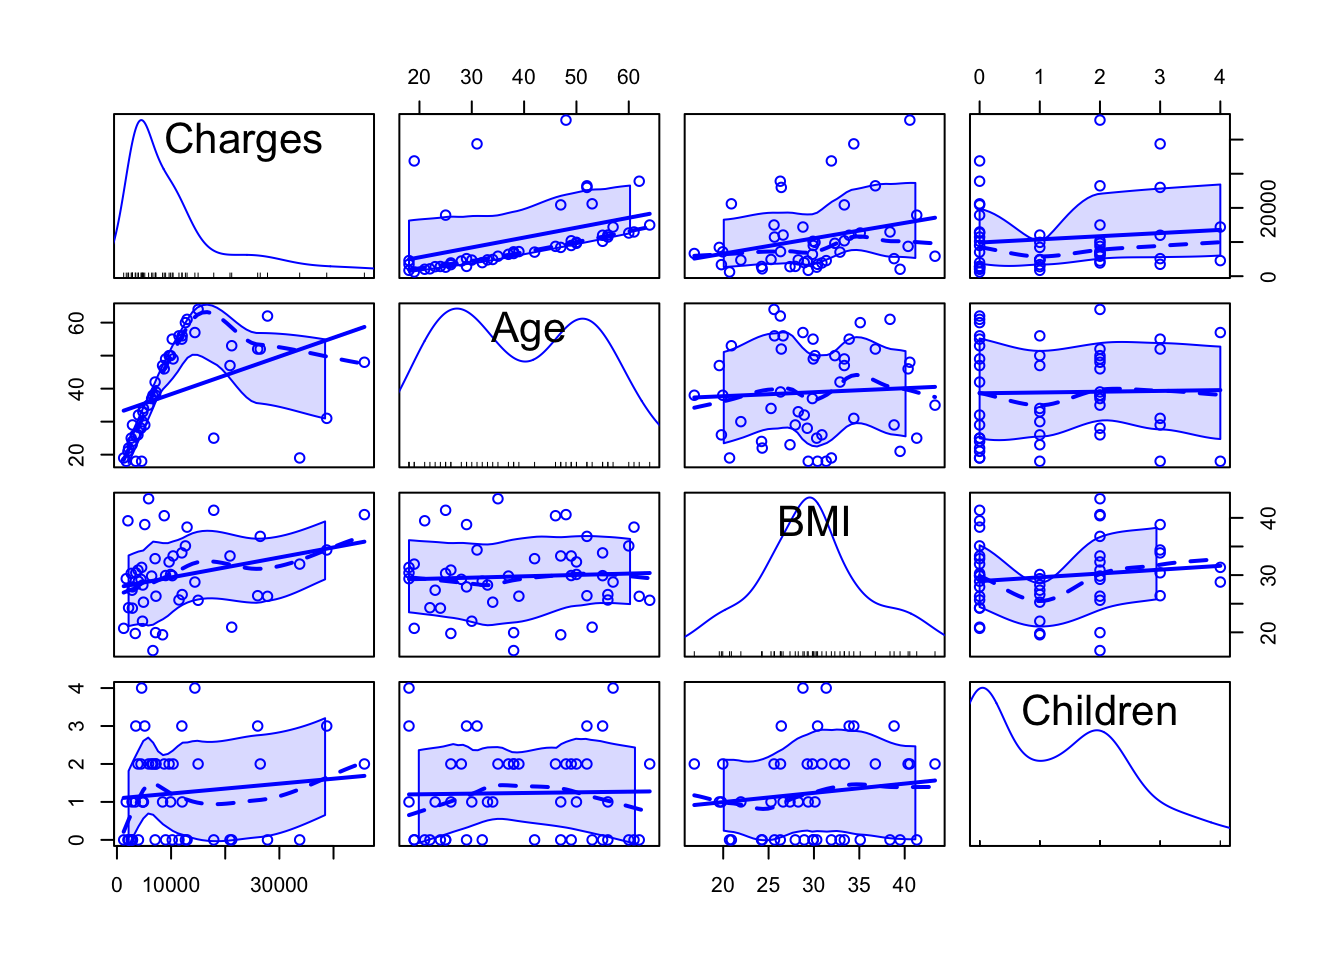
\includegraphics{CodingAssignment03_files/figure-latex/unnamed-chunk-1-1.pdf}
The quantitative variables are Charges, Age, BMI, Children. The
correlation between all quantitative variables is shown above. Based on
the data above, Age is positively correlated to Charges. As well as, BMI
and Charges, Children and Charges. Insurance Premiums would increase
based on an increase in age, BMI and to some small degree the number of
children you have.

\hypertarget{question-3}{%
\subsection{Question 3}\label{question-3}}

Run a regression that includes all independent variables in the data
table. Does the model above violate any of the Gauss-Markov assumptions?
If so, what are they and what is the solution for correcting?

\begin{Shaded}
\begin{Highlighting}[]
\NormalTok{model }\OtherTok{\textless{}{-}} \FunctionTok{lm}\NormalTok{(Charges}\SpecialCharTok{\textasciitilde{}}\NormalTok{ Age }\SpecialCharTok{+}\NormalTok{ BMI }\SpecialCharTok{+}\NormalTok{ Female }\SpecialCharTok{+}\NormalTok{ Children }\SpecialCharTok{+}\NormalTok{ Smoker }\SpecialCharTok{+}\NormalTok{WinterSprings }\SpecialCharTok{+}\NormalTok{ WinterPark }\SpecialCharTok{+}\NormalTok{ Oviedo, }\AttributeTok{data =}\NormalTok{ insuranceremove3)}
\FunctionTok{summary}\NormalTok{(model)}
\end{Highlighting}
\end{Shaded}

\begin{verbatim}
## 
## Call:
## lm(formula = Charges ~ Age + BMI + Female + Children + Smoker + 
##     WinterSprings + WinterPark + Oviedo, data = insuranceremove3)
## 
## Residuals:
##     Min      1Q  Median      3Q     Max 
## -8097.0 -2816.0  -833.3  1299.2 16597.4 
## 
## Coefficients:
##                Estimate Std. Error t value Pr(>|t|)    
## (Intercept)   -10562.11    4330.65  -2.439  0.01951 *  
## Age              228.91      52.23   4.383 8.94e-05 ***
## BMI              357.59     119.86   2.983  0.00496 ** 
## Female          -934.12    1577.27  -0.592  0.55720    
## Children         835.30     680.73   1.227  0.22734    
## Smoker         24141.19    2506.00   9.633 9.54e-12 ***
## WinterSprings     97.83    2089.80   0.047  0.96291    
## WinterPark     -3892.00    1961.23  -1.984  0.05446 .  
## Oviedo         -1311.73    2238.58  -0.586  0.56136    
## ---
## Signif. codes:  0 '***' 0.001 '**' 0.01 '*' 0.05 '.' 0.1 ' ' 1
## 
## Residual standard error: 4932 on 38 degrees of freedom
## Multiple R-squared:  0.8039, Adjusted R-squared:  0.7626 
## F-statistic: 19.47 on 8 and 38 DF,  p-value: 2.993e-11
\end{verbatim}

\begin{Shaded}
\begin{Highlighting}[]
\FunctionTok{par}\NormalTok{(}\AttributeTok{mfrow=}\FunctionTok{c}\NormalTok{(}\DecValTok{1}\NormalTok{,}\DecValTok{2}\NormalTok{))}
\FunctionTok{hist}\NormalTok{(train}\SpecialCharTok{$}\NormalTok{Charges) }\CommentTok{\#before}

\NormalTok{train}\SpecialCharTok{$}\NormalTok{lnCharges }\OtherTok{\textless{}{-}} \FunctionTok{log}\NormalTok{(train}\SpecialCharTok{$}\NormalTok{Charges)}

\FunctionTok{hist}\NormalTok{(train}\SpecialCharTok{$}\NormalTok{lnCharges) }\CommentTok{\#after}
\end{Highlighting}
\end{Shaded}

\includegraphics{CodingAssignment03_files/figure-latex/unnamed-chunk-2-1.pdf}

\begin{Shaded}
\begin{Highlighting}[]
\FunctionTok{hist}\NormalTok{(train}\SpecialCharTok{$}\NormalTok{Age)}
\NormalTok{train}\SpecialCharTok{$}\NormalTok{lnAge }\OtherTok{\textless{}{-}} \FunctionTok{log}\NormalTok{(train}\SpecialCharTok{$}\NormalTok{Age)}

\FunctionTok{hist}\NormalTok{(train}\SpecialCharTok{$}\NormalTok{lnAge)}
\end{Highlighting}
\end{Shaded}

\includegraphics{CodingAssignment03_files/figure-latex/unnamed-chunk-2-2.pdf}

\begin{Shaded}
\begin{Highlighting}[]
\FunctionTok{hist}\NormalTok{(train}\SpecialCharTok{$}\NormalTok{Children)}
\NormalTok{train}\SpecialCharTok{$}\NormalTok{lnChildren }\OtherTok{\textless{}{-}} \FunctionTok{log}\NormalTok{(train}\SpecialCharTok{$}\NormalTok{Children)}

\FunctionTok{hist}\NormalTok{(train}\SpecialCharTok{$}\NormalTok{lnChildren)}
\end{Highlighting}
\end{Shaded}

\includegraphics{CodingAssignment03_files/figure-latex/unnamed-chunk-2-3.pdf}

\begin{Shaded}
\begin{Highlighting}[]
\FunctionTok{hist}\NormalTok{(train}\SpecialCharTok{$}\NormalTok{BMI)}
\NormalTok{train}\SpecialCharTok{$}\NormalTok{lnBMI }\OtherTok{\textless{}{-}} \FunctionTok{log}\NormalTok{(train}\SpecialCharTok{$}\NormalTok{BMI)}

\FunctionTok{hist}\NormalTok{(train}\SpecialCharTok{$}\NormalTok{lnBMI)}
\end{Highlighting}
\end{Shaded}

\includegraphics{CodingAssignment03_files/figure-latex/unnamed-chunk-2-4.pdf}

\begin{Shaded}
\begin{Highlighting}[]
\FunctionTok{scatterplotMatrix}\NormalTok{(train[,}\FunctionTok{c}\NormalTok{(}\DecValTok{1}\NormalTok{,}\DecValTok{2}\NormalTok{,}\DecValTok{3}\NormalTok{,}\DecValTok{5}\NormalTok{)]) }
\end{Highlighting}
\end{Shaded}

\includegraphics{CodingAssignment03_files/figure-latex/unnamed-chunk-2-5.pdf}
Charges is not normally distributed and Age is a bimodal distribution
which violates the third Gauss-Markov assumption because it is not a
linear relationship. By transforming the data with a log relationship
this will fix the assumption violation.

\hypertarget{question-4}{%
\subsection{Question 4}\label{question-4}}

Implement the solutions from question 3, such as data transformation,
along with any other changes you wish. Use the sample data and run a new
regression. How have the fit measures changed? How have the signs and
significance of the coefficients changed?

\begin{Shaded}
\begin{Highlighting}[]
\FunctionTok{par}\NormalTok{(}\AttributeTok{mfrow=}\FunctionTok{c}\NormalTok{(}\DecValTok{2}\NormalTok{,}\DecValTok{2}\NormalTok{))}
\FunctionTok{plot}\NormalTok{(train}\SpecialCharTok{$}\NormalTok{Charges)}

\FunctionTok{par}\NormalTok{(}\AttributeTok{mfrow=}\FunctionTok{c}\NormalTok{(}\DecValTok{2}\NormalTok{,}\DecValTok{2}\NormalTok{))}
\end{Highlighting}
\end{Shaded}

\includegraphics{CodingAssignment03_files/figure-latex/q3-1.pdf}

\begin{Shaded}
\begin{Highlighting}[]
\FunctionTok{plot}\NormalTok{(train}\SpecialCharTok{$}\NormalTok{Age)}

\NormalTok{model\_1 }\OtherTok{\textless{}{-}} \FunctionTok{lm}\NormalTok{(train}\SpecialCharTok{$}\NormalTok{lnCharges }\SpecialCharTok{\textasciitilde{}}\NormalTok{., }\AttributeTok{data =}\NormalTok{ train[,}\FunctionTok{c}\NormalTok{(}\DecValTok{2}\NormalTok{,}\DecValTok{3}\NormalTok{,}\DecValTok{5}\NormalTok{,}\DecValTok{10}\NormalTok{)] )}

\FunctionTok{summary}\NormalTok{(model\_1)}
\end{Highlighting}
\end{Shaded}

\begin{verbatim}
## 
## Call:
## lm(formula = train$lnCharges ~ ., data = train[, c(2, 3, 5, 10)])
## 
## Residuals:
##     Min      1Q  Median      3Q     Max 
## -0.8056 -0.3910 -0.1889  0.1363  2.3272 
## 
## Coefficients:
##             Estimate Std. Error t value Pr(>|t|)    
## (Intercept) 6.321946   0.528252  11.968 8.52e-15 ***
## Age         0.040380   0.006997   5.771 9.92e-07 ***
## BMI         0.031654   0.015278   2.072   0.0448 *  
## Children    0.106636   0.084141   1.267   0.2124    
## ---
## Signif. codes:  0 '***' 0.001 '**' 0.01 '*' 0.05 '.' 0.1 ' ' 1
## 
## Residual standard error: 0.6439 on 40 degrees of freedom
## Multiple R-squared:  0.5062, Adjusted R-squared:  0.4691 
## F-statistic: 13.67 on 3 and 40 DF,  p-value: 2.782e-06
\end{verbatim}

\begin{Shaded}
\begin{Highlighting}[]
\FunctionTok{tbl\_regression}\NormalTok{(model\_1,}
               \AttributeTok{estimate\_fun =}  \SpecialCharTok{\textasciitilde{}}\FunctionTok{style\_sigfig}\NormalTok{(.x, }\AttributeTok{digits =} \DecValTok{4}\NormalTok{)) }\SpecialCharTok{\%\textgreater{}\%} \FunctionTok{as\_gt}\NormalTok{() }\SpecialCharTok{\%\textgreater{}\%}
\NormalTok{  gt}\SpecialCharTok{::}\FunctionTok{tab\_source\_note}\NormalTok{(gt}\SpecialCharTok{::}\FunctionTok{md}\NormalTok{(}\FunctionTok{paste0}\NormalTok{(}\StringTok{"Adjusted R{-}Squared: "}\NormalTok{,}\FunctionTok{round}\NormalTok{(}\FunctionTok{summary}\NormalTok{(model\_1)}\SpecialCharTok{$}\NormalTok{adj.r.squared}\SpecialCharTok{*} \DecValTok{100}\NormalTok{,}\AttributeTok{digits =} \DecValTok{2}\NormalTok{),}\StringTok{"\%"}\NormalTok{)))}
\end{Highlighting}
\end{Shaded}

\begin{verbatim}
## Registered S3 methods overwritten by 'broom':
##   method            from  
##   tidy.glht         jtools
##   tidy.summary.glht jtools
\end{verbatim}

\setlength{\LTpost}{0mm}
\begin{longtable}{lccc}
\toprule
\textbf{Characteristic} & \textbf{Beta} & \textbf{95\% CI}\textsuperscript{1} & \textbf{p-value} \\ 
\midrule
Age & 0.0404 & 0.0262, 0.0545 & <0.001 \\ 
BMI & 0.0317 & 0.0008, 0.0625 & 0.045 \\ 
Children & 0.1066 & -0.0634, 0.2767 & 0.2 \\ 
\bottomrule
\end{longtable}
\begin{minipage}{\linewidth}
\textsuperscript{1}CI = Confidence Interval\\
Adjusted R-Squared: 46.91\%\\
\end{minipage}

\begin{Shaded}
\begin{Highlighting}[]
\FunctionTok{par}\NormalTok{(}\AttributeTok{mfrow=}\FunctionTok{c}\NormalTok{(}\DecValTok{2}\NormalTok{,}\DecValTok{2}\NormalTok{))}
\end{Highlighting}
\end{Shaded}

\includegraphics{CodingAssignment03_files/figure-latex/q3-2.pdf}

\begin{Shaded}
\begin{Highlighting}[]
\FunctionTok{plot}\NormalTok{(model\_1)}
\end{Highlighting}
\end{Shaded}

\includegraphics{CodingAssignment03_files/figure-latex/q3-3.pdf}

\begin{Shaded}
\begin{Highlighting}[]
\NormalTok{model\_2 }\OtherTok{\textless{}{-}} \FunctionTok{lm}\NormalTok{(train}\SpecialCharTok{$}\NormalTok{lnAge }\SpecialCharTok{\textasciitilde{}}\NormalTok{., }\AttributeTok{data =}\NormalTok{ train[,}\FunctionTok{c}\NormalTok{(}\DecValTok{2}\NormalTok{,}\DecValTok{3}\NormalTok{,}\DecValTok{5}\NormalTok{,}\DecValTok{11}\NormalTok{)] )}

\FunctionTok{summary}\NormalTok{(model\_2)}
\end{Highlighting}
\end{Shaded}

\begin{verbatim}
## 
## Call:
## lm(formula = train$lnAge ~ ., data = train[, c(2, 3, 5, 11)])
## 
## Residuals:
##      Min       1Q   Median       3Q      Max 
## -0.15760 -0.03059  0.01405  0.04902  0.07152 
## 
## Coefficients:
##               Estimate Std. Error t value Pr(>|t|)    
## (Intercept)  2.5348890  0.0515834  49.142   <2e-16 ***
## Age          0.0270857  0.0006833  39.642   <2e-16 ***
## BMI         -0.0001930  0.0014919  -0.129    0.898    
## Children     0.0078977  0.0082163   0.961    0.342    
## ---
## Signif. codes:  0 '***' 0.001 '**' 0.01 '*' 0.05 '.' 0.1 ' ' 1
## 
## Residual standard error: 0.06288 on 40 degrees of freedom
## Multiple R-squared:  0.9753, Adjusted R-squared:  0.9734 
## F-statistic: 525.4 on 3 and 40 DF,  p-value: < 2.2e-16
\end{verbatim}

\begin{Shaded}
\begin{Highlighting}[]
\FunctionTok{tbl\_regression}\NormalTok{(model\_2,}
               \AttributeTok{estimate\_fun =}  \SpecialCharTok{\textasciitilde{}}\FunctionTok{style\_sigfig}\NormalTok{(.x, }\AttributeTok{digits =} \DecValTok{4}\NormalTok{)) }\SpecialCharTok{\%\textgreater{}\%} \FunctionTok{as\_gt}\NormalTok{() }\SpecialCharTok{\%\textgreater{}\%}
\NormalTok{  gt}\SpecialCharTok{::}\FunctionTok{tab\_source\_note}\NormalTok{(gt}\SpecialCharTok{::}\FunctionTok{md}\NormalTok{(}\FunctionTok{paste0}\NormalTok{(}\StringTok{"Adjusted R{-}Squared: "}\NormalTok{,}\FunctionTok{round}\NormalTok{(}\FunctionTok{summary}\NormalTok{(model\_2)}\SpecialCharTok{$}\NormalTok{adj.r.squared}\SpecialCharTok{*} \DecValTok{100}\NormalTok{,}\AttributeTok{digits =} \DecValTok{2}\NormalTok{),}\StringTok{"\%"}\NormalTok{)))}
\end{Highlighting}
\end{Shaded}

\setlength{\LTpost}{0mm}
\begin{longtable}{lccc}
\toprule
\textbf{Characteristic} & \textbf{Beta} & \textbf{95\% CI}\textsuperscript{1} & \textbf{p-value} \\ 
\midrule
Age & 0.0271 & 0.0257, 0.0285 & <0.001 \\ 
BMI & -0.0002 & -0.0032, 0.0028 & 0.9 \\ 
Children & 0.0079 & -0.0087, 0.0245 & 0.3 \\ 
\bottomrule
\end{longtable}
\begin{minipage}{\linewidth}
\textsuperscript{1}CI = Confidence Interval\\
Adjusted R-Squared: 97.34\%\\
\end{minipage}

\begin{Shaded}
\begin{Highlighting}[]
\FunctionTok{par}\NormalTok{(}\AttributeTok{mfrow=}\FunctionTok{c}\NormalTok{(}\DecValTok{2}\NormalTok{,}\DecValTok{2}\NormalTok{))}
\FunctionTok{plot}\NormalTok{(model\_2)}
\end{Highlighting}
\end{Shaded}

\includegraphics{CodingAssignment03_files/figure-latex/q3-4.pdf} When
comparing the original model vs.~model\_2 the adjusted R-square
increased from .76 to .97. Similarly, the P-value increased from
2.993e-11 to 2.2e-16. Therefore, there is a significant increase in the
fit of our model.

\hypertarget{question-5}{%
\subsection{Question 5}\label{question-5}}

Use the 3 withheld observations and calculate the performance measures
for your best two models. Which is the better model? (remember that
``better'' depends on whether your outlook is short or long run)

\begin{Shaded}
\begin{Highlighting}[]
\NormalTok{test}\SpecialCharTok{$}\NormalTok{lnCharges }\OtherTok{\textless{}{-}} \FunctionTok{log}\NormalTok{(test}\SpecialCharTok{$}\NormalTok{Charges)}
\NormalTok{test}\SpecialCharTok{$}\NormalTok{lnAge }\OtherTok{\textless{}{-}} \FunctionTok{log}\NormalTok{(test}\SpecialCharTok{$}\NormalTok{Age)}
\NormalTok{test}\SpecialCharTok{$}\NormalTok{AgeSquared }\OtherTok{\textless{}{-}}\NormalTok{ test}\SpecialCharTok{$}\NormalTok{Age}\SpecialCharTok{\^{}}\DecValTok{2}

\NormalTok{test}\SpecialCharTok{$}\NormalTok{model\_1 }\OtherTok{\textless{}{-}} \FunctionTok{predict}\NormalTok{(model\_1, }\AttributeTok{newdata =}\NormalTok{ test)}

\NormalTok{test}\SpecialCharTok{$}\NormalTok{model\_2 }\OtherTok{\textless{}{-}} \FunctionTok{predict}\NormalTok{(model\_2,}\AttributeTok{newdata =}\NormalTok{ test) }\SpecialCharTok{\%\textgreater{}\%} \FunctionTok{exp}\NormalTok{()}

\NormalTok{test}\SpecialCharTok{$}\NormalTok{errormodel\_1 }\OtherTok{\textless{}{-}}\NormalTok{ test}\SpecialCharTok{$}\NormalTok{model\_1 }\SpecialCharTok{{-}}\NormalTok{ test}\SpecialCharTok{$}\NormalTok{Charges}

\NormalTok{test}\SpecialCharTok{$}\NormalTok{errormodel\_2 }\OtherTok{\textless{}{-}}\NormalTok{ test}\SpecialCharTok{$}\NormalTok{model\_2 }\SpecialCharTok{{-}}\NormalTok{ test}\SpecialCharTok{$}\NormalTok{Charges}


\FunctionTok{mean}\NormalTok{(test}\SpecialCharTok{$}\NormalTok{errormodel\_1)}
\end{Highlighting}
\end{Shaded}

\begin{verbatim}
## [1] -8604.038
\end{verbatim}

\begin{Shaded}
\begin{Highlighting}[]
\FunctionTok{mean}\NormalTok{(test}\SpecialCharTok{$}\NormalTok{errormodel\_2)}
\end{Highlighting}
\end{Shaded}

\begin{verbatim}
## [1] -8571.367
\end{verbatim}

\begin{Shaded}
\begin{Highlighting}[]
\NormalTok{mae }\OtherTok{\textless{}{-}} \ControlFlowTok{function}\NormalTok{(error\_vector)\{}
\NormalTok{  error\_vector }\SpecialCharTok{\%\textgreater{}\%} 
  \FunctionTok{abs}\NormalTok{() }\SpecialCharTok{\%\textgreater{}\%} 
  \FunctionTok{mean}\NormalTok{()}
\NormalTok{\}}


\FunctionTok{mae}\NormalTok{(test}\SpecialCharTok{$}\NormalTok{errormodel\_1)}
\end{Highlighting}
\end{Shaded}

\begin{verbatim}
## [1] 8604.038
\end{verbatim}

\begin{Shaded}
\begin{Highlighting}[]
\FunctionTok{mae}\NormalTok{(test}\SpecialCharTok{$}\NormalTok{errormodel\_2)}
\end{Highlighting}
\end{Shaded}

\begin{verbatim}
## [1] 8571.367
\end{verbatim}

\begin{Shaded}
\begin{Highlighting}[]
\NormalTok{rmse }\OtherTok{\textless{}{-}} \ControlFlowTok{function}\NormalTok{(error\_vector)\{}
\NormalTok{   error\_vector}\SpecialCharTok{\^{}}\DecValTok{2} \SpecialCharTok{\%\textgreater{}\%} 
  \FunctionTok{mean}\NormalTok{() }\SpecialCharTok{\%\textgreater{}\%} 
  \FunctionTok{sqrt}\NormalTok{()}

\NormalTok{\}}


\FunctionTok{rmse}\NormalTok{(test}\SpecialCharTok{$}\NormalTok{errormodel\_1)}
\end{Highlighting}
\end{Shaded}

\begin{verbatim}
## [1] 9360.858
\end{verbatim}

\begin{Shaded}
\begin{Highlighting}[]
\FunctionTok{rmse}\NormalTok{(test}\SpecialCharTok{$}\NormalTok{errormodel\_2)}
\end{Highlighting}
\end{Shaded}

\begin{verbatim}
## [1] 9325.077
\end{verbatim}

\begin{Shaded}
\begin{Highlighting}[]
\NormalTok{mape }\OtherTok{\textless{}{-}} \ControlFlowTok{function}\NormalTok{(error\_vector, actual\_vector)\{}
\NormalTok{  (error\_vector}\SpecialCharTok{/}\NormalTok{actual\_vector) }\SpecialCharTok{\%\textgreater{}\%} 
    \FunctionTok{abs}\NormalTok{() }\SpecialCharTok{\%\textgreater{}\%} 
    \FunctionTok{mean}\NormalTok{()}
\NormalTok{\}}


\FunctionTok{mape}\NormalTok{(test}\SpecialCharTok{$}\NormalTok{errormodel\_1, test}\SpecialCharTok{$}\NormalTok{Charges)}
\end{Highlighting}
\end{Shaded}

\begin{verbatim}
## [1] 0.9986186
\end{verbatim}

\begin{Shaded}
\begin{Highlighting}[]
\FunctionTok{mape}\NormalTok{(test}\SpecialCharTok{$}\NormalTok{errormodel\_2, test}\SpecialCharTok{$}\NormalTok{Age)}
\end{Highlighting}
\end{Shaded}

\begin{verbatim}
## [1] 206.6201
\end{verbatim}

\begin{Shaded}
\begin{Highlighting}[]
\NormalTok{potential1 }\OtherTok{\textless{}{-}} \FunctionTok{data.frame}\NormalTok{(}\AttributeTok{Age =} \DecValTok{60}\NormalTok{,}
                            \AttributeTok{BMI =} \DecValTok{22}\NormalTok{,}
                            \AttributeTok{Children =} \DecValTok{0}\NormalTok{,}
                            \AttributeTok{Female =} \DecValTok{1}\NormalTok{,}
                            \AttributeTok{Smoker =} \DecValTok{0}\NormalTok{,}
                            \AttributeTok{WinterSprings =} \DecValTok{0}\NormalTok{,}
                            \AttributeTok{WinterPark =} \DecValTok{0}\NormalTok{,}
                            \AttributeTok{Oviedo =} \DecValTok{1}\NormalTok{)}
\NormalTok{potential2 }\OtherTok{\textless{}{-}} \FunctionTok{data.frame}\NormalTok{(}\AttributeTok{Age =} \DecValTok{40}\NormalTok{,}
                            \AttributeTok{BMI =} \DecValTok{30}\NormalTok{,}
                            \AttributeTok{Children =} \DecValTok{1}\NormalTok{,}
                            \AttributeTok{Female =} \DecValTok{0}\NormalTok{,}
                            \AttributeTok{Smoker =} \DecValTok{0}\NormalTok{,}
                            \AttributeTok{WinterSprings =} \DecValTok{0}\NormalTok{,}
                            \AttributeTok{WinterPark =} \DecValTok{0}\NormalTok{,}
                            \AttributeTok{Oviedo =} \DecValTok{0}\NormalTok{)}
\NormalTok{potential3 }\OtherTok{\textless{}{-}} \FunctionTok{data.frame}\NormalTok{(}\AttributeTok{Age =} \DecValTok{25}\NormalTok{,}
                            \AttributeTok{BMI =} \DecValTok{25}\NormalTok{,}
                            \AttributeTok{Children =} \DecValTok{0}\NormalTok{,}
                            \AttributeTok{Female =} \DecValTok{0}\NormalTok{,}
                            \AttributeTok{Smoker =} \DecValTok{1}\NormalTok{,}
                            \AttributeTok{WinterSprings =} \DecValTok{0}\NormalTok{,}
                            \AttributeTok{WinterPark =} \DecValTok{1}\NormalTok{,}
                            \AttributeTok{Oviedo =} \DecValTok{0}\NormalTok{)}
\NormalTok{potential4 }\OtherTok{\textless{}{-}} \FunctionTok{data.frame}\NormalTok{(}\AttributeTok{Age =} \DecValTok{33}\NormalTok{,}
                            \AttributeTok{BMI =} \DecValTok{35}\NormalTok{,}
                            \AttributeTok{Children =} \DecValTok{2}\NormalTok{,}
                            \AttributeTok{Female =} \DecValTok{1}\NormalTok{,}
                            \AttributeTok{Smoker =} \DecValTok{0}\NormalTok{,}
                            \AttributeTok{WinterSprings =} \DecValTok{1}\NormalTok{,}
                            \AttributeTok{WinterPark =} \DecValTok{0}\NormalTok{,}
                            \AttributeTok{Oviedo =} \DecValTok{0}\NormalTok{)}
\NormalTok{potential5 }\OtherTok{\textless{}{-}} \FunctionTok{data.frame}\NormalTok{(}\AttributeTok{Age =} \DecValTok{45}\NormalTok{,}
                            \AttributeTok{BMI =} \DecValTok{27}\NormalTok{,}
                            \AttributeTok{Children =} \DecValTok{3}\NormalTok{,}
                            \AttributeTok{Female =} \DecValTok{1}\NormalTok{,}
                            \AttributeTok{Smoker =} \DecValTok{0}\NormalTok{,}
                            \AttributeTok{WinterSprings =} \DecValTok{0}\NormalTok{,}
                            \AttributeTok{WinterPark =} \DecValTok{0}\NormalTok{,}
                            \AttributeTok{Oviedo =} \DecValTok{1}\NormalTok{)}

\FunctionTok{predict}\NormalTok{(model\_2, }\AttributeTok{newdata =}\NormalTok{ potential1, }\AttributeTok{interval =} \StringTok{\textquotesingle{}prediction\textquotesingle{}}\NormalTok{)}
\end{Highlighting}
\end{Shaded}

\begin{verbatim}
##        fit      lwr      upr
## 1 4.155787 4.020759 4.290815
\end{verbatim}

\begin{Shaded}
\begin{Highlighting}[]
\FunctionTok{predict}\NormalTok{(model\_2, }\AttributeTok{newdata =}\NormalTok{ potential2, }\AttributeTok{interval =} \StringTok{\textquotesingle{}prediction\textquotesingle{}}\NormalTok{)}
\end{Highlighting}
\end{Shaded}

\begin{verbatim}
##        fit      lwr      upr
## 1 3.620425 3.491869 3.748982
\end{verbatim}

\begin{Shaded}
\begin{Highlighting}[]
\FunctionTok{predict}\NormalTok{(model\_2, }\AttributeTok{newdata =}\NormalTok{ potential3, }\AttributeTok{interval =} \StringTok{\textquotesingle{}prediction\textquotesingle{}}\NormalTok{)}
\end{Highlighting}
\end{Shaded}

\begin{verbatim}
##        fit      lwr      upr
## 1 3.207207 3.075516 3.338897
\end{verbatim}

\begin{Shaded}
\begin{Highlighting}[]
\FunctionTok{predict}\NormalTok{(model\_2, }\AttributeTok{newdata =}\NormalTok{ potential4, }\AttributeTok{interval =} \StringTok{\textquotesingle{}prediction\textquotesingle{}}\NormalTok{)}
\end{Highlighting}
\end{Shaded}

\begin{verbatim}
##        fit      lwr      upr
## 1 3.437758 3.307301 3.568214
\end{verbatim}

\begin{Shaded}
\begin{Highlighting}[]
\FunctionTok{predict}\NormalTok{(model\_2, }\AttributeTok{newdata =}\NormalTok{ potential5, }\AttributeTok{interval =} \StringTok{\textquotesingle{}prediction\textquotesingle{}}\NormalTok{)}
\end{Highlighting}
\end{Shaded}

\begin{verbatim}
##        fit      lwr      upr
## 1 3.772229 3.639374 3.905083
\end{verbatim}

\begin{verbatim}
# Based on our calculations, model_2 is the better performing model. Comparing the two models, Model_2 has a slightly lower mean, MAE, RMSE. However, the MAPE is significantly larger which does not support model_2.

## Question 6

Provide interpretations of the coefficients, do the signs make sense? Perform marginal change analysis (thing 2) on the independent variables.


```r
# The coefficients are significantly smaller in model_2, the sign in BMI is now negative but was not statistically significant in our model. 
\end{verbatim}

\hypertarget{question-7}{%
\subsection{Question 7}\label{question-7}}

An eager insurance representative comes back with five potential
clients. Using the better of the two models selected above, provide the
prediction intervals for the five potential clients using the
information provided by the insurance rep.

\begin{longtable}[]{@{}lllllll@{}}
\toprule()
Customer & Age & BMI & Female & Children & Smoker & City \\
\midrule()
\endhead
1 & 60 & 22 & 1 & 0 & 0 & Oviedo \\
2 & 40 & 30 & 0 & 1 & 0 & Sanford \\
3 & 25 & 25 & 0 & 0 & 1 & Winter Park \\
4 & 33 & 35 & 1 & 2 & 0 & Winter Springs \\
5 & 45 & 27 & 1 & 3 & 0 & Oviedo \\
\bottomrule()
\end{longtable}

\begin{Shaded}
\begin{Highlighting}[]
\NormalTok{potential1 }\OtherTok{\textless{}{-}} \FunctionTok{data.frame}\NormalTok{(}\AttributeTok{Age =} \DecValTok{60}\NormalTok{,}
                            \AttributeTok{BMI =} \DecValTok{22}\NormalTok{,}
                            \AttributeTok{Children =} \DecValTok{0}\NormalTok{,}
                            \AttributeTok{Female =} \DecValTok{1}\NormalTok{,}
                            \AttributeTok{Smoker =} \DecValTok{0}\NormalTok{,}
                            \AttributeTok{WinterSprings =} \DecValTok{0}\NormalTok{,}
                            \AttributeTok{WinterPark =} \DecValTok{0}\NormalTok{,}
                            \AttributeTok{Oviedo =} \DecValTok{1}\NormalTok{)}
\NormalTok{potential2 }\OtherTok{\textless{}{-}} \FunctionTok{data.frame}\NormalTok{(}\AttributeTok{Age =} \DecValTok{40}\NormalTok{,}
                            \AttributeTok{BMI =} \DecValTok{30}\NormalTok{,}
                            \AttributeTok{Children =} \DecValTok{1}\NormalTok{,}
                            \AttributeTok{Female =} \DecValTok{0}\NormalTok{,}
                            \AttributeTok{Smoker =} \DecValTok{0}\NormalTok{,}
                            \AttributeTok{WinterSprings =} \DecValTok{0}\NormalTok{,}
                            \AttributeTok{WinterPark =} \DecValTok{0}\NormalTok{,}
                            \AttributeTok{Oviedo =} \DecValTok{1}\NormalTok{)}
\NormalTok{potential3 }\OtherTok{\textless{}{-}} \FunctionTok{data.frame}\NormalTok{(}\AttributeTok{Age =} \DecValTok{25}\NormalTok{,}
                            \AttributeTok{BMI =} \DecValTok{25}\NormalTok{,}
                            \AttributeTok{Children =} \DecValTok{0}\NormalTok{,}
                            \AttributeTok{Female =} \DecValTok{0}\NormalTok{,}
                            \AttributeTok{Smoker =} \DecValTok{1}\NormalTok{,}
                            \AttributeTok{WinterSprings =} \DecValTok{0}\NormalTok{,}
                            \AttributeTok{WinterPark =} \DecValTok{1}\NormalTok{,}
                            \AttributeTok{Oviedo =} \DecValTok{0}\NormalTok{)}
\NormalTok{potential4 }\OtherTok{\textless{}{-}} \FunctionTok{data.frame}\NormalTok{(}\AttributeTok{Age =} \DecValTok{33}\NormalTok{,}
                            \AttributeTok{BMI =} \DecValTok{35}\NormalTok{,}
                            \AttributeTok{Children =} \DecValTok{2}\NormalTok{,}
                            \AttributeTok{Female =} \DecValTok{1}\NormalTok{,}
                            \AttributeTok{Smoker =} \DecValTok{0}\NormalTok{,}
                            \AttributeTok{WinterSprings =} \DecValTok{1}\NormalTok{,}
                            \AttributeTok{WinterPark =} \DecValTok{0}\NormalTok{,}
                            \AttributeTok{Oviedo =} \DecValTok{0}\NormalTok{)}
\NormalTok{potential5 }\OtherTok{\textless{}{-}} \FunctionTok{data.frame}\NormalTok{(}\AttributeTok{Age =} \DecValTok{45}\NormalTok{,}
                            \AttributeTok{BMI =} \DecValTok{27}\NormalTok{,}
                            \AttributeTok{Children =} \DecValTok{3}\NormalTok{,}
                            \AttributeTok{Female =} \DecValTok{1}\NormalTok{,}
                            \AttributeTok{Smoker =} \DecValTok{0}\NormalTok{,}
                            \AttributeTok{WinterSprings =} \DecValTok{0}\NormalTok{,}
                            \AttributeTok{WinterPark =} \DecValTok{0}\NormalTok{,}
                            \AttributeTok{Oviedo =} \DecValTok{1}\NormalTok{)}

\FunctionTok{predict}\NormalTok{(model\_2, }\AttributeTok{newdata =}\NormalTok{ potential1, }\AttributeTok{interval =} \StringTok{\textquotesingle{}prediction\textquotesingle{}}\NormalTok{)}
\end{Highlighting}
\end{Shaded}

\begin{verbatim}
##        fit      lwr      upr
## 1 4.155787 4.020759 4.290815
\end{verbatim}

\begin{Shaded}
\begin{Highlighting}[]
\FunctionTok{predict}\NormalTok{(model\_2, }\AttributeTok{newdata =}\NormalTok{ potential2, }\AttributeTok{interval =} \StringTok{\textquotesingle{}prediction\textquotesingle{}}\NormalTok{)}
\end{Highlighting}
\end{Shaded}

\begin{verbatim}
##        fit      lwr      upr
## 1 3.620425 3.491869 3.748982
\end{verbatim}

\begin{Shaded}
\begin{Highlighting}[]
\FunctionTok{predict}\NormalTok{(model\_2, }\AttributeTok{newdata =}\NormalTok{ potential3, }\AttributeTok{interval =} \StringTok{\textquotesingle{}prediction\textquotesingle{}}\NormalTok{)}
\end{Highlighting}
\end{Shaded}

\begin{verbatim}
##        fit      lwr      upr
## 1 3.207207 3.075516 3.338897
\end{verbatim}

\begin{Shaded}
\begin{Highlighting}[]
\FunctionTok{predict}\NormalTok{(model\_2, }\AttributeTok{newdata =}\NormalTok{ potential4, }\AttributeTok{interval =} \StringTok{\textquotesingle{}prediction\textquotesingle{}}\NormalTok{)}
\end{Highlighting}
\end{Shaded}

\begin{verbatim}
##        fit      lwr      upr
## 1 3.437758 3.307301 3.568214
\end{verbatim}

\begin{Shaded}
\begin{Highlighting}[]
\FunctionTok{predict}\NormalTok{(model\_2, }\AttributeTok{newdata =}\NormalTok{ potential5, }\AttributeTok{interval =} \StringTok{\textquotesingle{}prediction\textquotesingle{}}\NormalTok{)}
\end{Highlighting}
\end{Shaded}

\begin{verbatim}
##        fit      lwr      upr
## 1 3.772229 3.639374 3.905083
\end{verbatim}

\begin{verbatim}
   fit     lwr      upr
\end{verbatim}

1 4.171419 4.02813 4.314709 fit lwr upr 1 3.612978 3.477785 3.748172 fit
lwr upr 1 3.204361 3.066025 3.342697 fit lwr upr 1 3.415488 3.27815
3.552825 fit lwr upr 1 3.753567 3.614209 3.892924

\hypertarget{question-8}{%
\subsection{Question 8}\label{question-8}}

The owner notices that some of the predictions are wider than others,
explain why.

\hypertarget{by-looking-at-the-prediction-values-used-in-the-model-the-values-are-outside-the-normal-mean-used-to-test-the-model-therefore-the-values-would-be-outside-what-we-expect-potentially-causing-a-wider-prediction-interval.}{%
\section{By looking at the prediction values used in the model the
values are outside the normal mean used to test the model therefore, the
values would be outside what we expect potentially causing a wider
prediction
interval.}\label{by-looking-at-the-prediction-values-used-in-the-model-the-values-are-outside-the-normal-mean-used-to-test-the-model-therefore-the-values-would-be-outside-what-we-expect-potentially-causing-a-wider-prediction-interval.}}

If predictions vary very widely it could be due to issues with model
specification bias or not including the qualitative data when devising a
model therefore the values included when predicting the models will not
be as efficient.

\hypertarget{question-9}{%
\subsection{Question 9}\label{question-9}}

Are there any prediction problems that occur with the five potential
clients? If so, explain.

Prediction problems occur when the model doesn't take into consideration
qualitative variables such as location or when factors used in the
predictions such as AGE, BMI are outside the normal variables used to
develop the model.

\end{document}
